% Paperformat
\documentclass[a4paper, 12pt]{scrartcl}
\usepackage{cite}
\usepackage{ragged2e}
\usepackage{url}
\usepackage{bm} % bold math
\usepackage{nccmath} % medium fraction with mfrac 
\usepackage{amssymb}
\usepackage{graphicx}
\usepackage{amsthm} % theorems
\usepackage{hyperref}
\usepackage{float}

\newtheorem{theorem}{Theorem}[section]
\begin{document}

\begin{titlepage}
	\vspace*{\stretch{1}}
	\begin{center}
		{\Large\bfseries Bachelor Thesis}           \\[6.5ex]
		
		{\huge\bfseries Visualizing Dynamic Programming on Tree Decompositions}                  \\[6.5ex]
		
		\vspace{6ex}
				
		\textsc{\Large Martin Röbke}    \\[3ex]
		{\Large born: 04.03.1995 in Dresden, Germany}    \\[2ex]
		{\Large matriculation number: 3949819}    \\[2ex]
		{\Large martin.roebke@tu-dresden.de}    \\[2ex]
		\textsc{\large 
			}             \\[12ex]
		\vfill
		{\Large Technische Universität Dresden}               \\
		Faculty of Computer Science \\
		International Center For Computational Logic 		\\[5ex]
		
		{\Large Supervisor: Dr. Johannes Fichte}\\[2ex]
		{\Large Second evaluator:  Prof. Dr. rer. nat. Stefan Gumhold}\\[5ex]
		
		\vfill
		Dresden, \today
	\end{center}
	\vspace{\stretch{2}}
\end{titlepage}



\section*{Abstract}
\vspace{4ex}
The thesis is about a practical and lightweight implementation for visualizing dynamic programming on tree decompositions.
I created the python-package\href{https://pypi.org/project/tdvisu}{tdvisu} for the purpose of visualizing, teaching and analyzing the solving process of MSOL-problems using tree decomposition. 
Intended audience: Developer of dynamic programming on tree decompositions for debugging. Researcher of such algorithms for comparisons and visualizations.
Teachers or students wanting some automatic visualization of their examples and the dynamic-solving-process.
As two reference implementations of dynamic programming on tree decompositions the projects \href{https://github.com/daajoe/GPUSAT}{GPUSAT} and \href{https://github.com/hmarkus/dp_on_dbs}{dpdb} were chosen.



\newpage

%  table
\tableofcontents

% chapter on next page
\newpage


\section{Introduction}
Graphs are increasingly interesting in scientific work.
The idea for this project comes from my supervisor Dr. Johannes Fichte, who works on and with many projects such as the ones listed above on solving monadic second order logic (MSOL\cite{Courcelle2012}) problems using highly parallelized architectures like graphics processing units or state of the art databases.
One early implementation is published in \cite{evaluationMSO} where for different real world examples the results looked promising
These projects are very competitive ????REF????? for solving even large instances of those problems.

intro. mit motivation und related work, state of the art, advancements.


Visualization Pipeline

Stand Umsetzung, Tools: Slack, Trello, GitHub, Presentations

\newpage
\section{Background}

\subsection{Boolean satisfiability problem}
\url{https://en.wikipedia.org/wiki/Boolean_satisfiability_problem}

SAT was the first known NP-complete problem, as proved by Stephen Cook at the University of Toronto in 1971 \cite{SAT1971}

\begin{align*}
\text{literal}&\equiv\text{boolean variable v or its negation} \\
\text{clause}&\equiv\text{finite set of literals, interpreted as the disjunction} \\
\text{unit}&\equiv\text{clause with $|$c$|$=1} \\
\text{CNF formula}&\equiv\text{set of clauses, interpreted as their conjunction} \\
\text{var}&\equiv\text{set of variables contained in the clause or clause set C} \\
\text{assignment}&\equiv \text{$\alpha $:var(C) $\to $ \{0,1\}} \\
\text{satisfiedclause}&\equiv\text{if $\exists $v $\in $ var(c), v$\in $c and $\alpha $(v)=1 or $\neg $v$\in $c and $\alpha $(v)= 0. Otherwise falsified}\\ 
\text{satisfiedform}&\equiv\text{each clause in the formula is satisfied by assignment} \\
\end{align*}

Connection to graphs with ...DA...



\subsection{MSOL}
See also figure~\ref{fig:logictheory}.
\subsection{DIMACS Format}
\subsection{Tree Decomposition}
\subsection{Courcelle's Theorem}
\begin{quotation}
	Every graph property definable in monadic second-order logic (MSO) is decidable in linear time on graphs of bounded treewidth.\\
	{\small Courcelle, Bruno (1990)}\footnote{Courcelle, Bruno "The monadic second-order logic of graphs. I. Recognizable sets of finite graphs",\\ Information and Computation, 85 (1990) no. 1: 12-75}
\end{quotation}

For all $k \in \mathbb{N}$ and MSO-sentences F is the decision problem for a given graph G, whether $G \models F$ is true, in time $2^{p(tw(G))} \cdot |G|$ with a polynom p decidable.
\begin{itemize}
	
	\item \emph{drawback:} still expensive ($2^{p(tw G)}$, $2^{2^{(\#Q)}}$, large constants) \smallskip 

\end{itemize}

The workflow then looks like we see in figure~\ref{fig:UsageCourcelle}.

\begin{figure}[H]
	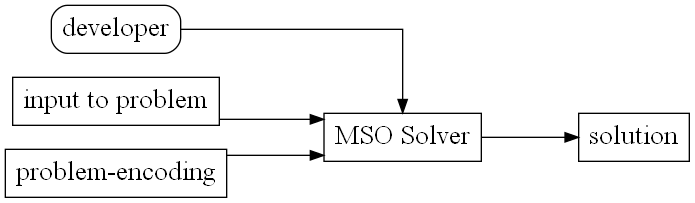
\includegraphics[height=0.2\textheight]{images/UsageCourcelle.gv.png}
	\caption{Implementation of the theorem}
	\label{fig:UsageCourcelle}
\end{figure}

\newpage
\section{Concept}
What I do and why I did it
Steps in Trello, Issues, Commits
Research: language (python - explain) graph-construction (graphviz vs networkX), examples (diploma at first). 
\newpage
\section{My Visualization Project}

Github
Objectives
htd hier oder auslassen?
Files / Classes / Methods
Current 
perspective 
Checking with www.deepcode.ai

\newpage
\subsection{Integration in GPUSAT}
Programm
Umsetzung
Beispiel
\newpage
\subsection{Integration in dpdb}
Programm
Umsetzung
Beispiel
\newpage
\section{Application and Images }
\newpage
\section{Summary and Outline}
What is achieved?
What worked good, what bad?
\bibliography{bibtex}{}
\bibliographystyle{ieeetr}

\newpage
\appendix
\section{Images}
\begin{figure}[H]
	\centering
	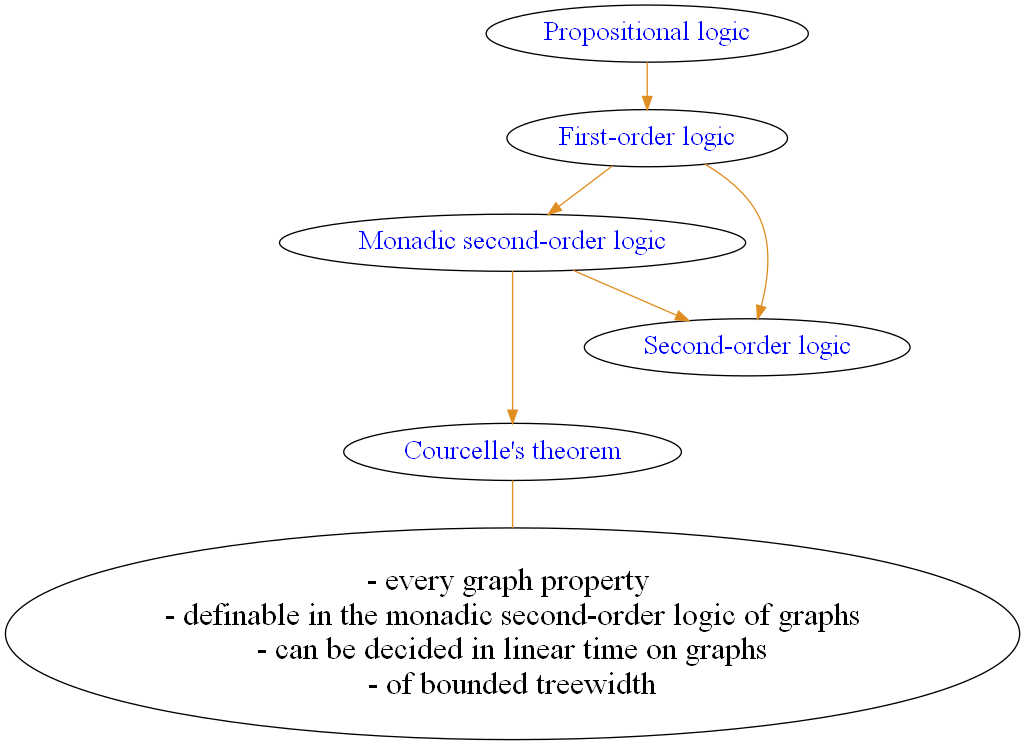
\includegraphics[width=0.8\linewidth]{images/logictheory.png}
	\caption{From propositional logic to monadic second order logic}
	\label{fig:logictheory}
\end{figure}
\end{document}